\documentclass[12pt]{article}
\usepackage[paperwidth=25cm,paperheight=17cm,margin=1.4cm]{geometry}
\usepackage[T1]{fontenc}
\usepackage[utf8]{inputenc}
\usepackage[magyar]{babel}
\usepackage{lmodern}
\usepackage{amsmath,amssymb}
\usepackage{enumitem}
\usepackage{array}
\usepackage{tikz}
\usetikzlibrary{arrows.meta,decorations.pathmorphing,patterns,calc}
\usepackage{pgfplots}
\pgfplotsset{compat=1.16}
\usepackage[most]{tcolorbox}

\pagestyle{empty}
\setlength{\parindent}{0pt}
\setlength{\parskip}{4pt}
\setlist[itemize]{leftmargin=1.4em, itemsep=3pt, topsep=2pt, parsep=0pt}

\newcommand{\dia}[1]{\newpage{\Large\bfseries #1}\par\vspace{2pt}{\color{blue!50!black}\hrule height 1pt}\vspace{8pt}}

\newtcolorbox{pelda}[1][]{colback=green!4,colframe=green!45!black,fonttitle=\bfseries,
  title=Kidolgozott példa,left=5pt,right=5pt,top=3pt,bottom=3pt,before skip=6pt,after skip=4pt,#1}
\newtcolorbox{fontos}[1][]{colback=blue!3,colframe=blue!45!black,
  left=5pt,right=5pt,top=3pt,bottom=3pt,before skip=6pt,after skip=4pt,#1}

\begin{document}

%====================================================================
\begin{center}
  \vspace*{1.2cm}
  {\Huge\bfseries Rezgések és mechanikai hullámok}\\[1.4cm]
\end{center}

\begin{center}
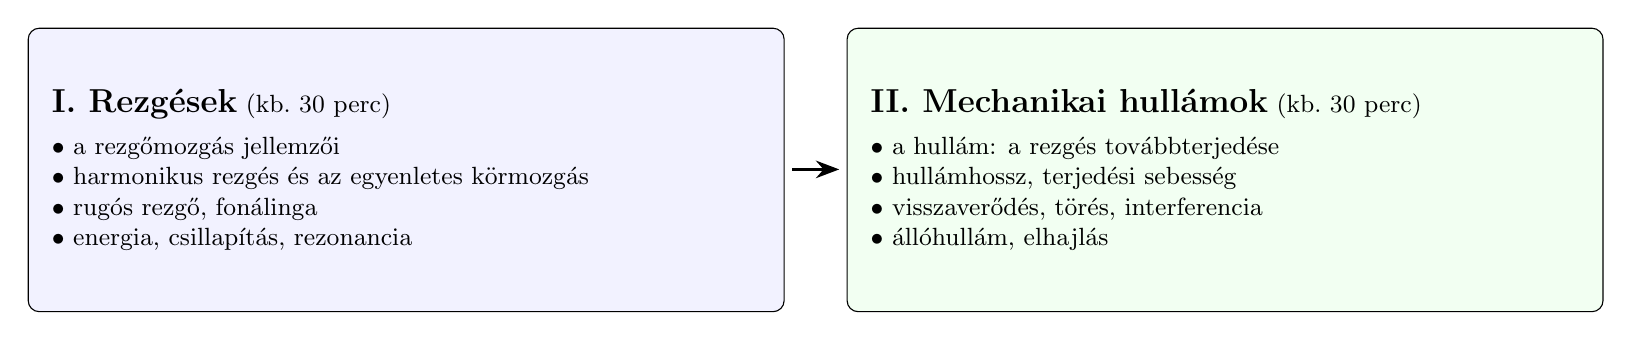
\begin{tikzpicture}[font=\small,
    resz/.style={draw,rounded corners,minimum width=9.6cm,minimum height=3.6cm,align=left,anchor=north},
    >=Stealth]
  \node[resz,fill=blue!5] (r) at (-5.2,0) {%
    \parbox{9cm}{\textbf{\large I.\ Rezgések} (kb.\ 30 perc)\\[4pt]
    $\bullet$ a rezgőmozgás jellemzői\\
    $\bullet$ harmonikus rezgés és az egyenletes körmozgás\\
    $\bullet$ rugós rezgő, fonálinga\\
    $\bullet$ energia, csillapítás, rezonancia}};
  \node[resz,fill=green!5] (h) at (5.2,0) {%
    \parbox{9cm}{\textbf{\large II.\ Mechanikai hullámok} (kb.\ 30 perc)\\[4pt]
    $\bullet$ a hullám: a rezgés továbbterjedése\\
    $\bullet$ hullámhossz, terjedési sebesség\\
    $\bullet$ visszaverődés, törés, interferencia\\
    $\bullet$ állóhullám, elhajlás}};
  \draw[->,very thick] (-0.3,-1.8) -- (0.3,-1.8);
\end{tikzpicture}
\end{center}

\vspace{1.0cm}
\begin{fontos}
\centering Miért most? Az előző két órán sokszor használtuk a hullámokat (rács, kétréses
kísérlet, de Broglie-állóhullám). Ma megnézzük, \textbf{mi is az a rezgés és a hullám}, a
legszemléletesebb esetben: rugón, kötélen, vízen és levegőben.
\end{fontos}

%====================================================================
\dia{1. A rezgőmozgás és jellemzői}

\begin{minipage}[t]{0.52\linewidth}\vspace{0pt}
\begin{itemize}
  \item \textbf{Rezgőmozgás:} egy test egy egyensúlyi helyzet körül ismétlődően ide-oda mozog
    (rugóra akasztott test, inga, hangvilla ága, gitárhúr, óra billegője).
  \item A mozgást a \textbf{kitérés--idő} grafikonnal írjuk le. Ha ez szinuszgörbe, a rezgés
    \textbf{harmonikus}.
\end{itemize}
\begin{fontos}
\renewcommand{\arraystretch}{1.35}
\begin{tabular}{@{}l>{\raggedright\arraybackslash}p{6.4cm}@{}}
\textbf{kitérés} ($y$) & pillanatnyi távolság az egyensúlyi helyzettől \\
\textbf{amplitúdó} ($A$) & a legnagyobb kitérés \\
\textbf{periódusidő} ($T$) & egy teljes rezgés ideje \\
\textbf{frekvencia} ($f$) & rezgésszám 1~s alatt: $f = \dfrac1T$, \; $[f] = \text{Hz}$ \\
\textbf{körfrekvencia} ($\omega$) & $\omega = 2\pi f = \dfrac{2\pi}{T}$
\end{tabular}
\end{fontos}
\end{minipage}\hfill
\begin{minipage}[t]{0.45\linewidth}\vspace{0pt}\centering
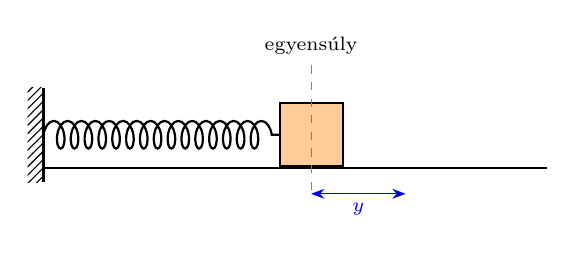
\begin{tikzpicture}[>=Stealth,font=\small]
  \fill[pattern=north east lines] (-0.2,-0.6) rectangle (0,0.6);
  \draw[thick] (0,-0.6) -- (0,0.6);
  \draw[decorate,decoration={coil,aspect=0.5,segment length=5pt,amplitude=5pt},thick] (0,0) -- (3.0,0);
  \draw[thick,fill=orange!40] (3.0,-0.4) rectangle (3.8,0.4);
  \draw[thick] (0,-0.42) -- (6.4,-0.42);
  \draw[dashed,gray] (3.4,-0.7) -- (3.4,0.9) node[above,font=\scriptsize,black] {egyensúly};
  \draw[<->,blue] (3.4,-0.75) -- node[below,font=\scriptsize] {$y$} (4.6,-0.75);
\end{tikzpicture}

\vspace{8pt}
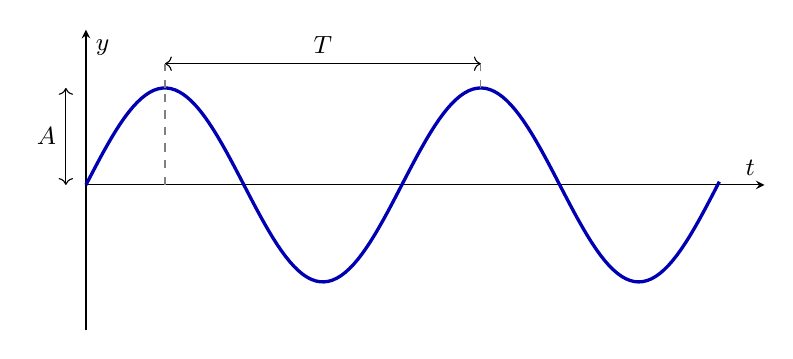
\begin{tikzpicture}
\begin{axis}[width=10.2cm,height=5.4cm,axis lines=middle,xmin=0,xmax=13.5,ymin=-1.5,ymax=1.6,
    xlabel={$t$},ylabel={$y$},xtick=\empty,ytick=\empty,
    label style={font=\small},clip=false]
  \addplot[very thick,blue!70!black,domain=0:12.6,samples=150] {sin(deg(x))};
  \draw[dashed,gray] (axis cs:1.571,0) -- (axis cs:1.571,1);
  \draw[<->] (axis cs:-0.4,0) -- node[left,font=\small] {$A$} (axis cs:-0.4,1);
  \draw[<->] (axis cs:1.571,1.25) -- node[above,font=\small] {$T$} (axis cs:7.854,1.25);
  \draw[dashed,gray] (axis cs:7.854,1) -- (axis cs:7.854,1.25);
  \draw[dashed,gray] (axis cs:1.571,1) -- (axis cs:1.571,1.25);
\end{axis}
\end{tikzpicture}
\end{minipage}

%====================================================================
\dia{2. A harmonikus rezgés: az egyenletes körmozgás vetülete}

\begin{minipage}[t]{0.52\linewidth}\vspace{0pt}
\begin{itemize}
  \item Ha egy pont $A$ sugarú körön $\omega$ szögsebességgel egyenletesen kering, a
    \textbf{függőleges vetülete} éppen harmonikus rezgést végez. (Ezt pl.\ egy forgó
    korong csapjának árnyékával lehet megmutatni.)
  \item A vetítésből kapjuk a kitérést, a sebességet és a gyorsulást:
\end{itemize}
\begin{fontos}
\[ y = A\sin(\omega t), \qquad v = A\omega\cos(\omega t), \qquad a = -A\omega^2\sin(\omega t) \]
\[ v_\text{max} = A\omega, \qquad a_\text{max} = A\omega^2, \qquad
   \boxed{a = -\omega^2 y} \]
\end{fontos}
\begin{itemize}
  \item Az \textbf{egyensúlyi helyzetben} a sebesség maximális, a gyorsulás nulla.
  \item A \textbf{szélső helyzetekben} a sebesség nulla, a gyorsulás maximális, és mindig az
    egyensúlyi helyzet felé mutat.
\end{itemize}
\end{minipage}\hfill
\begin{minipage}[t]{0.45\linewidth}\vspace{0pt}\centering
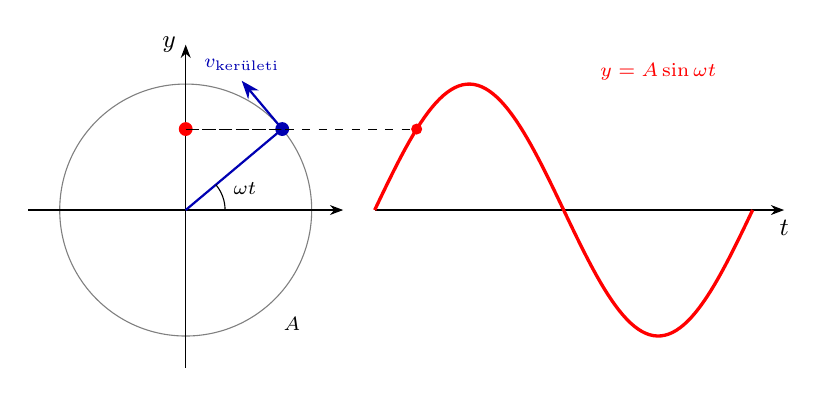
\begin{tikzpicture}[>=Stealth,font=\small]
  \draw[gray] (0,0) circle (1.6);
  \draw[->] (-2,0) -- (2,0);
  \draw[->] (0,-2) -- (0,2.1) node[left] {$y$};
  \coordinate (P) at (40:1.6);
  \draw[thick,blue!70!black] (0,0) -- (P);
  \fill[blue!70!black] (P) circle (2.5pt);
  \draw (0.5,0) arc (0:40:0.5);
  \node at (0.75,0.27) {\scriptsize $\omega t$};
  \draw[dashed] (P) -- (0,{1.6*sin(40)});
  \fill[red] (0,{1.6*sin(40)}) circle (2.5pt);
  \draw[->,thick,blue!70!black] (P) -- ++(130:0.8) node[above,font=\scriptsize] {$v_\text{kerületi}$};
  % szinusz
  \draw[->] (2.4,0) -- (7.6,0) node[below] {$t$};
  \draw[very thick,red,domain=0:360,samples=100] plot ({2.4+\x/360*4.8},{1.6*sin(\x)});
  \draw[dashed] (0,{1.6*sin(40)}) -- ({2.4+40/360*4.8},{1.6*sin(40)});
  \fill[red] ({2.4+40/360*4.8},{1.6*sin(40)}) circle (2pt);
  \node[red,font=\scriptsize] at (6.0,1.75) {$y = A\sin\omega t$};
  \node[font=\scriptsize] at (1.35,-1.45) {$A$};
\end{tikzpicture}

\vspace{6pt}
{\small A körmozgás $\omega$ szögsebessége a rezgés \textbf{körfrekvenciája}. Egy kör
megtétele egy teljes rezgés, ezért $\omega = 2\pi/T$.}

\begin{fontos}[title=Fázis,fonttitle=\bfseries]
Ha a mozgás nem az egyensúlyi helyzetből indul: $\;y = A\sin(\omega t + \varphi_0)$.
Az $\omega t + \varphi_0$ szög a rezgés \textbf{fázisa}, $\varphi_0$ a \textbf{kezdőfázis}.
Két azonos frekvenciájú rezgés \textbf{azonos fázisú} ($\Delta\varphi = 0$), ha egyszerre érik
el ugyanazt a szélső helyzetet; \textbf{ellentétes fázisú} ($\Delta\varphi = \pi$, fél periódus
eltolódás), ha az egyik a felső, a másik az alsó szélső helyzetben van.
\end{fontos}
\end{minipage}

%====================================================================
\dia{3. Mitől harmonikus a rezgés? Rugós rezgő és fonálinga}

\begin{minipage}[t]{0.56\linewidth}\vspace{0pt}
\begin{itemize}
  \item A rezgés akkor harmonikus, ha a testre ható eredő erő \textbf{arányos a kitéréssel
    és vele ellentétes irányú} (\textbf{lineáris erőtörvény}):
    \[ F = -D\,y \]
    Rugónál $D$ a rugóállandó. Newton II.\ törvényéből $ma = -Dy$, és ezt $a = -\omega^2y$-nal
    összevetve:
\end{itemize}
\begin{fontos}
\[ \omega = \sqrt{\frac{D}{m}} \quad\Longrightarrow\quad
   \boxed{T = 2\pi\sqrt{\frac{m}{D}}} \quad\text{(rugós rezgő)} \]
\[ \boxed{T = 2\pi\sqrt{\frac{l}{g}}} \quad\text{(fonálinga, kis kitérésnél)} \]
\end{fontos}
\begin{itemize}
  \item A periódusidő \textbf{nem függ az amplitúdótól}. Ezért lehet ingával órát
    szabályozni.
  \item Nehezebb test lassabban rezeg, keményebb rugó gyorsabban. Az inga periódusideje nem
    függ a tömegtől, csak a hossztól (és $g$-től).
\end{itemize}
\end{minipage}\hfill
\begin{minipage}[t]{0.41\linewidth}\vspace{0pt}
\begin{pelda}
\textbf{Rugós rezgő:} $D = 40~\tfrac{\text{N}}{\text{m}}$, $m = 0{,}4$~kg, $A = 5$~cm.\\[3pt]
$\omega = \sqrt{\dfrac{40}{0{,}4}} = 10~\tfrac1{\text{s}}$, \quad
$T = \dfrac{2\pi}{\omega} \approx 0{,}63$~s, \quad $f \approx 1{,}6$~Hz\\[3pt]
$v_\text{max} = A\omega = 0{,}05\cdot 10 = 0{,}5~\tfrac{\text{m}}{\text{s}}$\\[2pt]
$a_\text{max} = A\omega^2 = 0{,}05\cdot 100 = 5~\tfrac{\text{m}}{\text{s}^2}$

\medskip
\textbf{Fonálinga:} $l = 1$~m:\\[2pt]
$T = 2\pi\sqrt{\dfrac{1}{9{,}8}}~\text{s} \approx 2{,}0$~s.
\end{pelda}

\centering
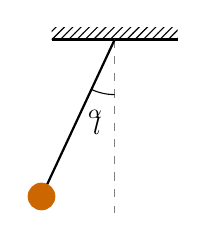
\begin{tikzpicture}[>=Stealth,font=\small]
  \fill[pattern=north east lines] (-0.8,0) rectangle (0.8,0.15);
  \draw[thick] (-0.8,0) -- (0.8,0);
  \draw[dashed,gray] (0,0) -- (0,-2.2);
  \draw[thick] (0,0) -- (-115:2.2);
  \fill[orange!80!black] (-115:2.2) circle (5pt);
  \draw (0,-0.7) arc (-90:-115:0.7);
  \node at (-0.25,-0.95) {\scriptsize $\alpha$};
  \node[right] at (-0.4,-1.1) {$l$};
\end{tikzpicture}
\end{minipage}

%====================================================================
\dia{4. A rezgés energiája}

\begin{minipage}[t]{0.52\linewidth}\vspace{0pt}
\begin{itemize}
  \item Rezgés közben a \textbf{mozgási} és a \textbf{rugalmas (helyzeti) energia} folyamatosan
    egymásba alakul, az összegük súrlódás nélkül állandó:
\end{itemize}
\begin{fontos}
\[ E = \tfrac12 mv^2 + \tfrac12 Dy^2 = \tfrac12 DA^2 = \tfrac12 m v_\text{max}^2 \]
\end{fontos}
\begin{itemize}
  \item Szélső helyzetben az energia csak rugalmas, az egyensúlyi helyzetben csak mozgási.
  \item Az energia az \textbf{amplitúdó négyzetével} arányos: kétszeres amplitúdó $\to$
    négyszeres energia.
  \item Egy tetszőleges helyen a sebesség az energiamegmaradásból:
    $v = \omega\sqrt{A^2 - y^2}$.
\end{itemize}
\begin{pelda}
Az előző rugós rezgőre: $E = \tfrac12\cdot 40\cdot 0{,}05^2 = 0{,}05$~J. Ellenőrzés:
$\tfrac12\cdot 0{,}4\cdot 0{,}5^2 = 0{,}05$~J. \checkmark\\
$y = 3$~cm-nél: $v = 10\cdot\sqrt{0{,}05^2 - 0{,}03^2} = 0{,}4~\tfrac{\text{m}}{\text{s}}$.
\end{pelda}
\end{minipage}\hfill
\begin{minipage}[t]{0.45\linewidth}\vspace{0pt}\centering
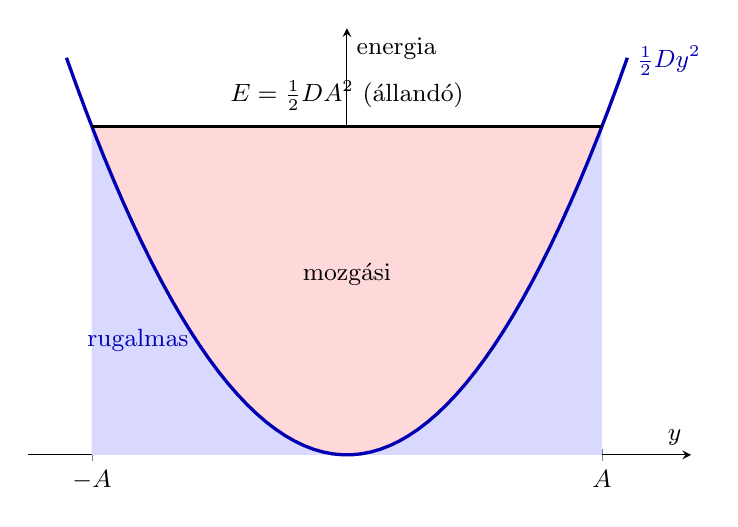
\begin{tikzpicture}
\begin{axis}[width=10cm,height=7cm,axis lines=middle,xmin=-1.25,xmax=1.35,ymin=0,ymax=1.3,
    xlabel={$y$},ylabel={energia},xtick={-1,0,1},xticklabels={$-A$,$0$,$A$},ytick=\empty,
    label style={font=\small},tick label style={font=\small},clip=false]
  \addplot[fill=red!15,draw=none,domain=-1:1,samples=60] {1} \closedcycle;
  \addplot[fill=blue!15,draw=none,domain=-1:1,samples=60] {x^2} \closedcycle;
  \addplot[very thick,blue!70!black,domain=-1.1:1.1,samples=60] {x^2};
  \addplot[very thick,black,domain=-1:1] {1};
  \node[font=\small] at (axis cs:0,0.55) {mozgási};
  \node[font=\small,blue!70!black] at (axis cs:-0.82,0.35) {rugalmas};
  \node[font=\small,anchor=south] at (axis cs:0,1.02) {$E = \tfrac12 DA^2$ (állandó)};
  \node[font=\small,blue!70!black,anchor=west] at (axis cs:1.1,1.2) {$\tfrac12 Dy^2$};
\end{axis}
\end{tikzpicture}
\end{minipage}

%====================================================================
\dia{5. Csillapított rezgés, kényszerrezgés, rezonancia}

\begin{minipage}[t]{0.50\linewidth}\vspace{0pt}
\begin{itemize}
  \item \textbf{Csillapított rezgés:} a valóságban súrlódás és közegellenállás miatt a
    rezgés energiája hővé alakul, az amplitúdó fokozatosan csökken.
  \item \textbf{Kényszerrezgés:} ha a rezgő rendszert egy külső, periodikus erő mozgatja, a
    rendszer \emph{a külső erő frekvenciájával} rezeg.
  \item \textbf{Rezonancia:} ha a gerjesztő frekvencia megegyezik a rendszer
    \textbf{saját frekvenciájával}, az amplitúdó nagyon nagyra nő. Ilyenkor a külső erő
    mindig ,,jó ütemben'' lök, így minden lökés növeli az energiát. Minél kisebb a
    csillapítás, annál magasabb és élesebb a csúcs.
\end{itemize}
\begin{fontos}
\textbf{Példák:} a hintát a saját ritmusában kell lökni. A centrifugázó mosógép egy
bizonyos fordulatszámnál erősen rázkódik. Hídon a katonák nem lépnek egyszerre. A
rádió hangolása is rezonancia: a vevő áramköre csak a kiválasztott frekvenciára
,,válaszol''.
\end{fontos}
\end{minipage}\hfill
\begin{minipage}[t]{0.47\linewidth}\vspace{0pt}\centering
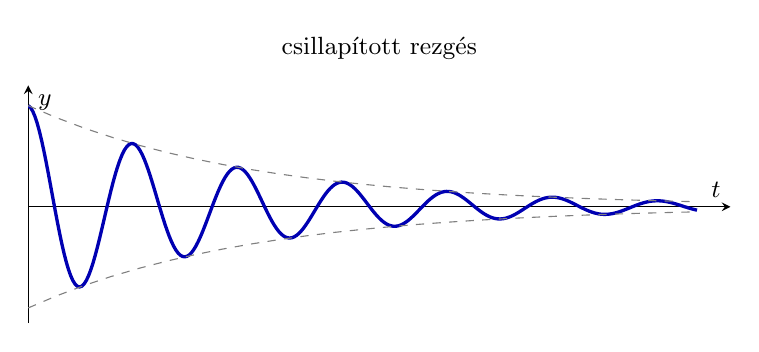
\begin{tikzpicture}
\begin{axis}[width=10.5cm,height=4.6cm,axis lines=middle,xmin=0,xmax=21,ymin=-1.15,ymax=1.2,
    xlabel={$t$},ylabel={$y$},xtick=\empty,ytick=\empty,label style={font=\small},
    title={\small csillapított rezgés}]
  \addplot[very thick,blue!70!black,domain=0:20,samples=300] {exp(-0.15*x)*cos(deg(2*x))};
  \addplot[dashed,gray,domain=0:20] {exp(-0.15*x)};
  \addplot[dashed,gray,domain=0:20] {-exp(-0.15*x)};
\end{axis}
\end{tikzpicture}

\vspace{2pt}
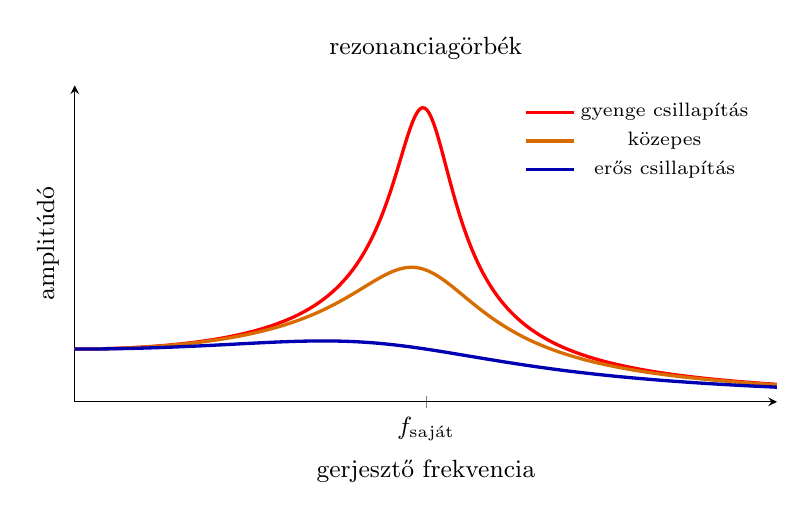
\begin{tikzpicture}
\begin{axis}[width=10.5cm,height=5.6cm,axis lines=left,xmin=0,xmax=2,ymin=0,ymax=6,
    xlabel={gerjesztő frekvencia},ylabel={amplitúdó},xtick={1},xticklabels={$f_\text{saját}$},
    ytick=\empty,label style={font=\small},tick label style={font=\small},
    title={\small rezonanciagörbék},
    legend style={font=\scriptsize,draw=none,fill=none,at={(0.98,0.98)},anchor=north east}]
  \addplot[very thick,red,domain=0:2,samples=300] {1/sqrt((1-x^2)^2+(0.18*x)^2)};
  \addplot[very thick,orange!85!black,domain=0:2,samples=200] {1/sqrt((1-x^2)^2+(0.4*x)^2)};
  \addplot[very thick,blue!70!black,domain=0:2,samples=200] {1/sqrt((1-x^2)^2+(1.0*x)^2)};
  \legend{gyenge csillapítás,közepes,erős csillapítás}
\end{axis}
\end{tikzpicture}
\end{minipage}

%====================================================================
\dia{6. Mi a hullám?}

\begin{minipage}[t]{0.52\linewidth}\vspace{0pt}
\begin{itemize}
  \item Ha egy rugalmas közeg egy pontját rezgésbe hozzuk, a rezgés a szomszédos részecskékre
    is átterjed: kialakul a \textbf{hullám}.
  \item \textbf{A hullám a rezgésállapotot és az energiát szállítja, nem az anyagot.} A
    közeg részecskéi csak a helyükön rezegnek. A vízen ringó falevél sem úszik el a
    hullámmal, csak fel-le mozog.
  \item \textbf{Transzverzális (keresztirányú) hullám:} a részecskék a terjedésre
    \emph{merőlegesen} rezegnek (kötélhullám, húron futó hullám).
  \item \textbf{Longitudinális (hosszanti) hullám:} a részecskék a terjedés
    \emph{irányában} rezegnek, sűrűsödések és ritkulások haladnak (hang a levegőben,
    rugóban futó lökés).
  \item A mechanikai hullámhoz \textbf{közeg kell}. Vákuumban nincs hang.
    (A fény elektromágneses hullám, annak nem kell közeg.)
\end{itemize}
\end{minipage}\hfill
\begin{minipage}[t]{0.45\linewidth}\vspace{0pt}\centering
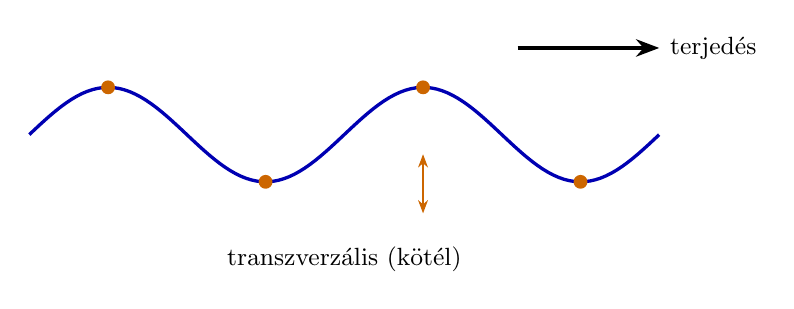
\begin{tikzpicture}[>=Stealth,font=\small]
  \draw[very thick,blue!70!black,domain=0:8,samples=120] plot (\x,{0.6*sin(\x*90)});
  \foreach \x in {1,3,5,7} \fill[orange!80!black] (\x,{0.6*sin(\x*90)}) circle (2.5pt);
  \draw[<->,orange!80!black] (5,-0.25) -- (5,-1.0);
  \draw[->,very thick] (6.2,1.1) -- (8,1.1) node[right] {terjedés};
  \node[below,font=\small] at (4,-1.3) {transzverzális (kötél)};
\end{tikzpicture}

\vspace{12pt}
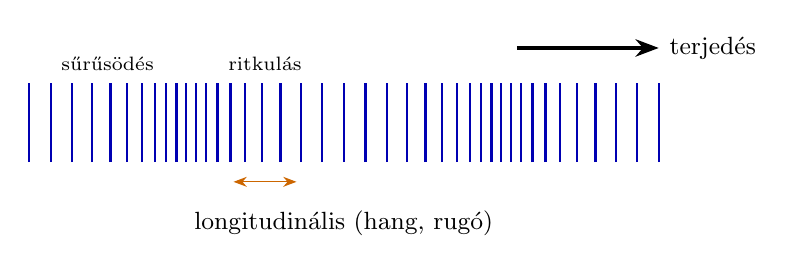
\begin{tikzpicture}[>=Stealth,font=\small]
  \foreach \i in {0,...,40}{
    \pgfmathsetmacro{\x}{\i*0.2 + 0.25*sin(\i*0.2*90)}
    \draw[thick,blue!70!black] (\x,-0.5) -- (\x,0.5);}
  \draw[<->,orange!80!black] (2.6,-0.75) -- (3.4,-0.75);
  \draw[->,very thick] (6.2,0.95) -- (8,0.95) node[right] {terjedés};
  \node[font=\scriptsize] at (1.0,0.75) {sűrűsödés};
  \node[font=\scriptsize] at (3.0,0.75) {ritkulás};
  \node[below,font=\small] at (4,-1.0) {longitudinális (hang, rugó)};
\end{tikzpicture}
\end{minipage}

%====================================================================
\dia{7. A hullám jellemzői: hullámhossz és terjedési sebesség}

\begin{minipage}[t]{0.50\linewidth}\vspace{0pt}
\begin{itemize}
  \item \textbf{Hullámhossz} ($\lambda$): két szomszédos, azonos rezgésállapotú pont távolsága
    (pl.\ két hullámhegyé). Egy periódusidő alatt a hullám éppen $\lambda$ utat tesz meg:
\end{itemize}
\begin{fontos}
\[ c = \frac{\lambda}{T} = \lambda f \]
\centering A \textbf{frekvenciát a forrás} szabja meg, a \textbf{terjedési sebességet a közeg}.
A hullámhossz ebből adódik.
\end{fontos}
\begin{itemize}
  \item Két grafikont nem szabad összekeverni: a \textbf{pillanatkép} (a kötél alakja egy
    adott pillanatban, $y$--$x$) és \textbf{egy pont mozgása} ($y$--$t$). Az elsőről a
    $\lambda$, a másodikról a $T$ olvasható le.
\end{itemize}
\begin{pelda}
Hang a levegőben ($c = 340~\tfrac{\text{m}}{\text{s}}$), $f = 440$~Hz (zenei ,,a''):
$\lambda = \dfrac{c}{f} = \dfrac{340}{440}~\text{m} \approx 0{,}77$~m. A hallható
tartomány ($20$~Hz--$20$~kHz) hullámhosszai $17$~m és $1{,}7$~cm között vannak.
\end{pelda}
\end{minipage}\hfill
\begin{minipage}[t]{0.47\linewidth}\vspace{0pt}\centering
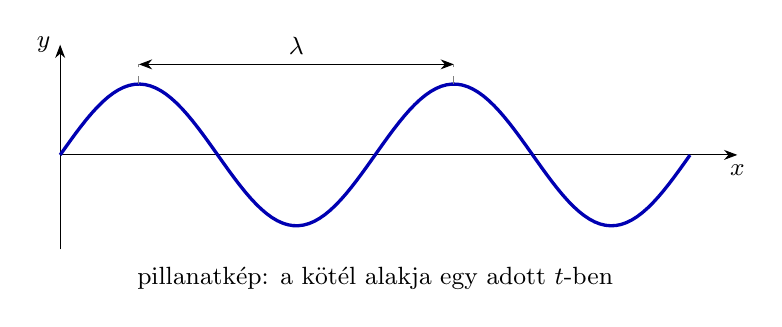
\begin{tikzpicture}[>=Stealth,font=\small]
  \draw[->] (0,0) -- (8.6,0) node[below] {$x$};
  \draw[->] (0,-1.2) -- (0,1.4) node[left] {$y$};
  \draw[very thick,blue!70!black,domain=0:8,samples=120] plot (\x,{0.9*sin(\x*90)});
  \draw[<->] (1,1.15) -- node[above] {$\lambda$} (5,1.15);
  \draw[dashed,gray] (1,0.9) -- (1,1.15);
  \draw[dashed,gray] (5,0.9) -- (5,1.15);
  \node[below,font=\small] at (4,-1.3) {pillanatkép: a kötél alakja egy adott $t$-ben};
\end{tikzpicture}

\vspace{14pt}
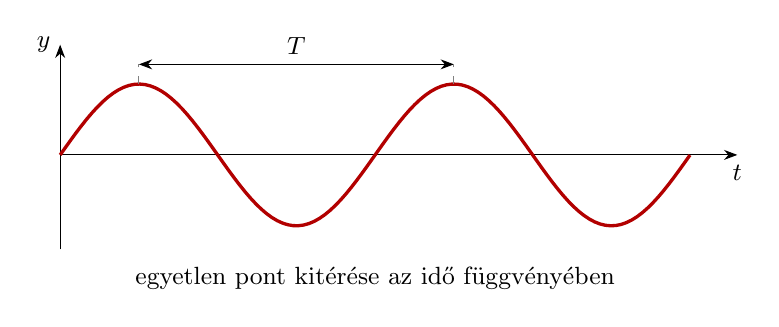
\begin{tikzpicture}[>=Stealth,font=\small]
  \draw[->] (0,0) -- (8.6,0) node[below] {$t$};
  \draw[->] (0,-1.2) -- (0,1.4) node[left] {$y$};
  \draw[very thick,red!70!black,domain=0:8,samples=120] plot (\x,{0.9*sin(\x*90)});
  \draw[<->] (1,1.15) -- node[above] {$T$} (5,1.15);
  \draw[dashed,gray] (1,0.9) -- (1,1.15);
  \draw[dashed,gray] (5,0.9) -- (5,1.15);
  \node[below,font=\small] at (4,-1.3) {egyetlen pont kitérése az idő függvényében};
\end{tikzpicture}
\end{minipage}

%====================================================================
\dia{8. Visszaverődés és törés}

\begin{minipage}[t]{0.50\linewidth}\vspace{0pt}
\textbf{Visszaverődés:} a közeg határán a hullám (részben) visszaverődik.
\begin{itemize}
  \item \textbf{Rögzített végről} (falhoz kötött kötél) a hullám \textbf{ellentétes
    fázisban} verődik vissza: a hullámhegyből hullámvölgy lesz.
  \item \textbf{Szabad végről} \textbf{azonos fázisban} verődik vissza.
  \item A beesési szög egyenlő a visszaverődési szöggel.
\end{itemize}
\textbf{Törés:} ha a hullám más terjedési sebességű közegbe ér, megváltozik az iránya.
\begin{fontos}
\[ \frac{\sin\alpha}{\sin\beta} = \frac{c_1}{c_2} = \frac{\lambda_1}{\lambda_2} \]
\centering A \textbf{frekvencia nem változik} (a forrás szabja meg), a sebesség és a
hullámhossz igen. Ahol lassabb a hullám, ott a beesési merőlegeshez \textbf{törik}.
\end{fontos}
{\small Példa: a vízhullám sekély vízben lassabb, ezért a part felé fordul, és a hullámfrontok
a parttal párhuzamosan érkeznek.}
\end{minipage}\hfill
\begin{minipage}[t]{0.47\linewidth}\vspace{0pt}\centering
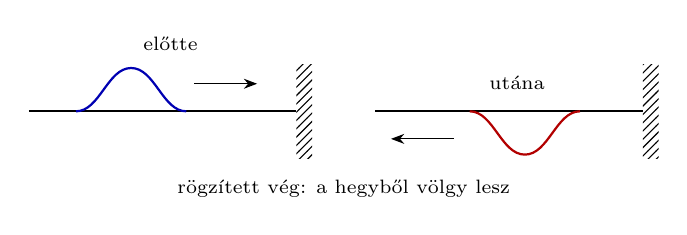
\begin{tikzpicture}[>=Stealth,font=\small]
  % rögzített vég
  \draw[thick] (0,0) -- (3.4,0);
  \fill[pattern=north east lines] (3.4,-0.6) rectangle (3.6,0.6);
  \draw[thick,blue!70!black] (0.6,0) .. controls (0.9,0) and (1.0,0.55) .. (1.3,0.55)
    .. controls (1.6,0.55) and (1.7,0) .. (2.0,0);
  \draw[->] (2.1,0.35) -- (2.9,0.35);
  \node[above,font=\scriptsize] at (1.8,0.65) {előtte};
  \draw[thick] (4.4,0) -- (7.8,0);
  \fill[pattern=north east lines] (7.8,-0.6) rectangle (8.0,0.6);
  \draw[thick,red!70!black] (5.6,0) .. controls (5.9,0) and (6.0,-0.55) .. (6.3,-0.55)
    .. controls (6.6,-0.55) and (6.7,0) .. (7.0,0);
  \draw[->] (5.4,-0.35) -- (4.6,-0.35);
  \node[above,font=\scriptsize] at (6.2,0.15) {utána};
  \node[below,font=\scriptsize] at (4,-0.75) {rögzített vég: a hegyből völgy lesz};
\end{tikzpicture}

\vspace{10pt}
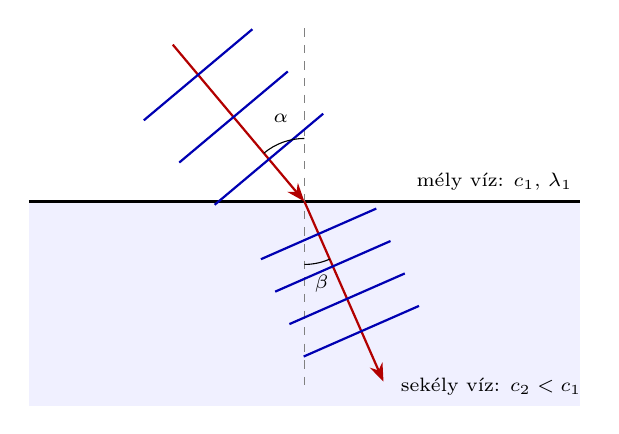
\begin{tikzpicture}[>=Stealth,font=\small]
  \fill[blue!6] (-3.5,-2.6) rectangle (3.5,0);
  \draw[thick] (-3.5,0) -- (3.5,0);
  \node[font=\scriptsize,anchor=west] at (1.3,0.25) {mély víz: $c_1$, $\lambda_1$};
  \node[font=\scriptsize,anchor=west] at (1.1,-2.35) {sekély víz: $c_2 < c_1$};
  \draw[dashed,gray] (0,2.2) -- (0,-2.4);
  % beeső hullámfrontok (merőlegesek a sugárra, sugár 40°-ban)
  \draw[->,thick,red!70!black] (130:2.6) -- (0,0);
  \foreach \d in {0.7,1.4,2.1}
    \draw[blue!70!black,thick] ($(130:\d)+(40:0.9)$) -- ($(130:\d)+(220:0.9)$);
  % megtört hullámfrontok, kisebb hullámhossz, sugár 23.7°-ban
  \draw[->,thick,red!70!black] (0,0) -- (-66.3:2.5);
  \foreach \d in {0.45,0.9,1.35,1.8}
    \draw[blue!70!black,thick] ($(-66.3:\d)+(23.7:0.8)$) -- ($(-66.3:\d)+(203.7:0.8)$);
  \draw (0,0.8) arc (90:130:0.8);
  \node at (-0.3,1.05) {\scriptsize $\alpha$};
  \draw (0,-0.8) arc (-90:-66.3:0.8);
  \node at (0.22,-1.05) {\scriptsize $\beta$};
\end{tikzpicture}
\end{minipage}

%====================================================================
\dia{9. Interferencia: hullámok találkozása}

\begin{minipage}[t]{0.55\linewidth}\vspace{0pt}
\begin{itemize}
  \item \textbf{Szuperpozíció:} ha két hullám találkozik, a kitérések
    \textbf{összeadódnak}, majd a hullámok zavartalanul haladnak tovább.
  \item Két \textbf{koherens} (azonos frekvenciájú, állandó fáziskülönbségű) forrás hullámai
    állandó \textbf{interferenciaképet} hoznak létre:
\end{itemize}
\begin{fontos}
\renewcommand{\arraystretch}{1.6}
\begin{tabular}{@{}ll@{}}
\textbf{erősítés:} & $\Delta s = k\lambda$ \quad ($k = 0, 1, 2, \dots$) \\
\textbf{kioltás:} & $\Delta s = (2k+1)\dfrac{\lambda}{2}$
\end{tabular}\\[2pt]
\centering ($\Delta s$: a két forrástól mért távolságok különbsége, az \textbf{útkülönbség})
\end{fontos}
\begin{itemize}
  \item Kioltásnál a hegy völgyre esik: \textbf{rezgés $+$ rezgés $=$ nyugalom}. Ez a
    hullámok jellegzetessége, ugyanaz, mint a fénynél (,,fény $+$ fény $=$ sötétség'').
  \item Az energia nem vész el, csak \emph{átrendeződik}: a kioltási helyekről hiányzó energia
    az erősítési helyeken jelenik meg.
\end{itemize}
\begin{pelda}
Két, azonos ütemben rezgő pálca vízhullámot kelt, $\lambda = 2$~cm. Egy pont az egyiktől
$10$~cm-re, a másiktól $13$~cm-re van: $\Delta s = 3~\text{cm} = 1{,}5\lambda$ $\Rightarrow$
ott a víz \textbf{nyugalomban} van.
\end{pelda}
\end{minipage}\hfill
\begin{minipage}[t]{0.42\linewidth}\vspace{0pt}\centering
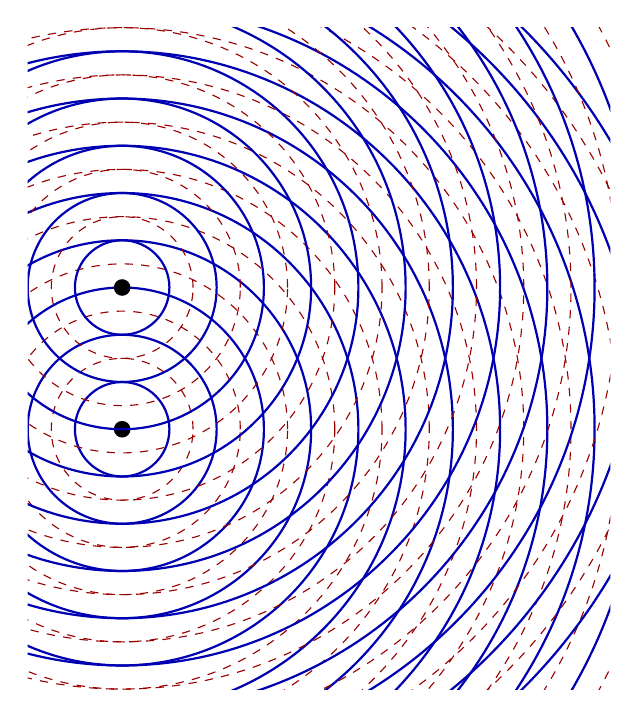
\begin{tikzpicture}[font=\small]
  \clip (-1.2,-4.2) rectangle (6.2,4.2);
  \foreach \s in {-0.9,0.9}{
    \foreach \r in {0.6,1.2,...,7.2}
      \draw[blue!70!black,thick] (0,\s) circle (\r);
    \foreach \r in {0.9,1.5,...,7.2}
      \draw[red!60!black,dashed] (0,\s) circle (\r);
    \fill (0,\s) circle (3pt);}
\end{tikzpicture}\\
{\small folytonos: hullámhegy, szaggatott: hullámvölgy.\\
Ahol két hegy (vagy két völgy) találkozik: erősítés;\\ahol hegy és völgy: kioltás.}
\end{minipage}

%====================================================================
\dia{10. Állóhullám}

\begin{minipage}[t]{0.52\linewidth}\vspace{0pt}
\begin{itemize}
  \item Ha a hullám egy rögzített végről visszaverődik, a beeső és a visszavert hullám
    interferenciájából \textbf{állóhullám} jön létre: a hullám nem halad. Vannak
    \textbf{csomópontok}, amelyek egyáltalán nem mozognak, és köztük
    \textbf{duzzadóhelyek}, ahol a legnagyobb a rezgés.
  \item Két szomszédos csomópont távolsága $\lambda/2$.
  \item \textbf{Két végén rögzített húron} csak olyan állóhullám alakulhat ki, amelynek
    a két végén csomópont van, vagyis a húr hossza a félhullámhossz egész számú
    többszöröse:
\end{itemize}
\begin{fontos}
\[ L = n\frac{\lambda}{2} \quad\Longrightarrow\quad f_n = n\frac{c}{2L}, \qquad n = 1, 2, 3, \dots \]
\centering $n = 1$: \textbf{alaphang}, $n \ge 2$: \textbf{felhangok} (az alaphang egész
számú többszörösei)
\end{fontos}
\begin{pelda}
Egy $L = 0{,}65$~m-es gitárhúr alaphangja $f_1 = 110$~Hz. A hullám sebessége a húron
$c = 2Lf_1 = 143~\tfrac{\text{m}}{\text{s}}$, az első felhang $f_2 = 220$~Hz.
\end{pelda}
{\small Ismerős? A de Broglie-féle atompályák ugyanígy ,,kvantáltak'': csak egész számú
hullám fér rájuk.}
\end{minipage}\hfill
\begin{minipage}[t]{0.45\linewidth}\vspace{0pt}\centering
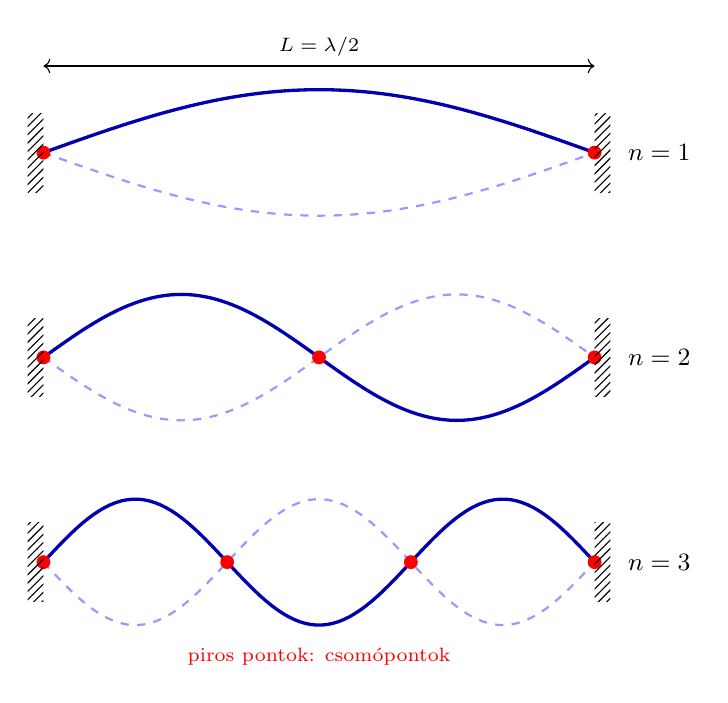
\begin{tikzpicture}[font=\small]
  \foreach \n/\yy in {1/0,2/-2.6,3/-5.2}{
    \begin{scope}[yshift=\yy cm]
      \draw[very thick,blue!70!black,domain=0:7,samples=100] plot (\x,{0.8*sin(\n*\x/7*180)});
      \draw[thick,blue!40,dashed,domain=0:7,samples=100] plot (\x,{-0.8*sin(\n*\x/7*180)});
      \foreach \k in {0,...,\n} \fill[red] ({7*\k/\n},0) circle (2.5pt);
      \fill[pattern=north east lines] (-0.2,-0.5) rectangle (0,0.5);
      \fill[pattern=north east lines] (7,-0.5) rectangle (7.2,0.5);
      \node[right] at (7.3,0) {$n=\n$};
    \end{scope}}
  \node[font=\scriptsize,red] at (3.5,-6.4) {piros pontok: csomópontok};
  \draw[<->] (0,1.1) -- node[above,font=\scriptsize] {$L = \lambda/2$} (7,1.1);
\end{tikzpicture}
\end{minipage}

%====================================================================
\dia{11. Huygens elve és az elhajlás}

\begin{minipage}[t]{0.52\linewidth}\vspace{0pt}
\begin{itemize}
  \item \textbf{Huygens--Fresnel-elv:} a hullámfront minden pontja újabb, elemi gömbhullámok
    (vízen körhullámok) forrása. A következő hullámfront ezeknek az elemi hullámoknak a
    burkolója. Ebből a visszaverődés és a törés törvénye is levezethető.
  \item \textbf{Elhajlás:} rés vagy akadály mögött a hullám az ,,árnyéktérbe'' is behatol.
    Az elhajlás akkor jelentős, ha a rés mérete \textbf{összemérhető a hullámhosszal}
    (vagy kisebb nála). Sokkal nagyobb résen a hullám szinte egyenesen halad át.
\end{itemize}
\begin{fontos}
\textbf{Miért halljuk a sarok mögül beszélőt, de miért nem látjuk?} A hang hullámhossza
($\sim 1$~m) összemérhető az ajtó és a fal méretével, ezért elhajlik. A fényé
($\sim 500$~nm) milliószor kisebb, ezért a fény egyenesen terjed, és éles árnyékot
ad. Elhajlást csak nagyon keskeny réseken mutat (optikai rács, előző óra!).
\end{fontos}
\end{minipage}\hfill
\begin{minipage}[t]{0.45\linewidth}\vspace{0pt}\centering
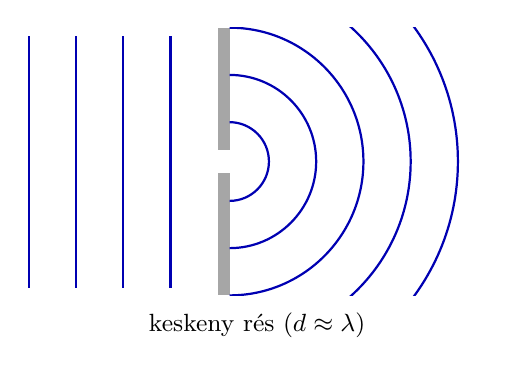
\begin{tikzpicture}[font=\small]
  \foreach \x in {-2.4,-1.8,...,-0.3} \draw[blue!70!black,thick] (\x,-1.6) -- (\x,1.6);
  \fill[gray!70] (0,0.15) rectangle (0.15,1.7);
  \fill[gray!70] (0,-1.7) rectangle (0.15,-0.15);
  \begin{scope}
    \clip (0.15,-1.7) rectangle (3.4,1.7);
    \foreach \r in {0.5,1.1,...,3.5} \draw[blue!70!black,thick] (0.15,0) circle (\r);
  \end{scope}
  \node[below] at (0.5,-1.8) {keskeny rés ($d \approx \lambda$)};
\end{tikzpicture}

\vspace{10pt}
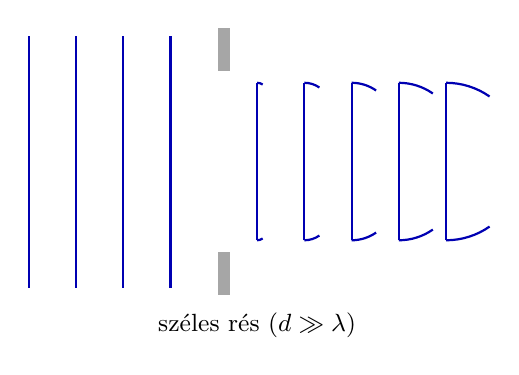
\begin{tikzpicture}[font=\small]
  \foreach \x in {-2.4,-1.8,...,-0.3} \draw[blue!70!black,thick] (\x,-1.6) -- (\x,1.6);
  \fill[gray!70] (0,1.15) rectangle (0.15,1.7);
  \fill[gray!70] (0,-1.7) rectangle (0.15,-1.15);
  \foreach \x in {0.5,1.1,...,3.2}{
    \draw[blue!70!black,thick] (\x,-1.0) -- (\x,1.0);
    \draw[blue!70!black,thick] (\x,1.0) arc (90:55:{(\x-0.15)*0.35});
    \draw[blue!70!black,thick] (\x,-1.0) arc (-90:-55:{(\x-0.15)*0.35});}
  \node[below] at (0.5,-1.8) {széles rés ($d \gg \lambda$)};
\end{tikzpicture}
\end{minipage}

%====================================================================
\dia{12. Összefoglalás}

\begin{minipage}[t]{0.50\linewidth}\vspace{0pt}
\begin{fontos}[title=Rezgések,fonttitle=\bfseries]
\renewcommand{\arraystretch}{1.55}
\begin{tabular}{@{}ll@{}}
jellemzők & $f = \dfrac1T$, \; $\omega = 2\pi f$ \\
harmonikus rezgés & $y = A\sin\omega t$, \; $a = -\omega^2y$ \\
maximumok & $v_\text{max} = A\omega$, \; $a_\text{max} = A\omega^2$ \\
rugós rezgő & $T = 2\pi\sqrt{m/D}$ \\
fonálinga & $T = 2\pi\sqrt{l/g}$ \\
energia & $E = \tfrac12 DA^2 = \tfrac12 mv_\text{max}^2$ \\
rezonancia & $f_\text{gerj} = f_\text{saját}$ \\
\end{tabular}
\end{fontos}
\end{minipage}\hfill
\begin{minipage}[t]{0.47\linewidth}\vspace{0pt}
\begin{fontos}[title=Hullámok,fonttitle=\bfseries,colback=green!3,colframe=green!45!black]
\renewcommand{\arraystretch}{1.55}
\begin{tabular}{@{}ll@{}}
terjedés & $c = \lambda f$ \; (energia, nem anyag) \\
törés & $\dfrac{\sin\alpha}{\sin\beta} = \dfrac{c_1}{c_2}$, \; $f$ állandó \\
erősítés & $\Delta s = k\lambda$ \\
kioltás & $\Delta s = (2k+1)\lambda/2$ \\
húr állóhulláma & $L = n\lambda/2$, \; $f_n = n\,c/(2L)$ \\
elhajlás & jelentős, ha a rés $\approx \lambda$ \\
\end{tabular}
\end{fontos}

\begin{fontos}[colback=yellow!8,colframe=orange!70!black,title=Házi feladat,fonttitle=\bfseries]
A \emph{gyakorló feladatsor} feladatai, és egy szóbeli tétel elmondása (3--4 perc).
\end{fontos}
\end{minipage}

\end{document}
